\chapter{python Porosity Uptake Correlator (pyPUC)}
\label{ch:pyPUC}

\newpage
\section*{Abstract}
For the optimal exploitation of porous materials in environmentally relevant \gls{physisorption} applications, the relationship between widths of pores within the \gls{adsorbent} and uptake capacity for the \gls{adsorbate} in question must be well understood. As these applications typically utilise the pressure-dependency of \gls{adsorption}, an understanding of the optimal pore size for uptake of the \gls{adsorbate} as a function of pressure is required. Current methods for investigating this relationship are currently limited by (i) reliance on computational modelling to approximate the result, (ii) only investigating this problem at a few discrete pressures, and often (iii) using the unsuitable measure of the `average' pore width. This work seeks to address all three of these inadequacies with the python Porosity Uptake Correlator; a software that uses experimental DataSets composed of gravimetric uptake isotherms and \acrfullpl{psd} of a group of samples that are compositionally similar, yet with diversity in terms of their porosity. Porosity (of all samples) within some pore size range is correlated to uptake of the \gls{adsorbate} at a given pressure \textit{via} linear regression. This process is then repeated for all defined pore size ranges and pressures, yielding a relationship between porosity within pores within some width range and association with improved uptake of the \gls{adsorbent} (defined by the Pearson coefficient, $r^2$).

In \ref{pub:pyPUC}, pyPUC was applied to the uptake of \ce{CO2} on \glspl{turbostratic carbon}, which gave some novel insights into this \gls{adsorption} process. Firstly, while \glspl{ultramicropore} are very important for low pressure \ce{CO2} uptake, at pressures above \qty{1.0}{\bar}, their influence diminishes significantly. However there is an indication that the traditional division of \glspl{micropore} into \glspl{ultramicropore} and \glspl{supermicropore} at \qty{7.0}{\angstrom} may not truly have physical significance to \ce{CO2} uptake. Finally, the comparative investigation of the utility of \ce{N2}, \ce{O2}, and \ce{H2} as well as the pairs \ce{N2}/\ce{H2}, and \ce{O2}/\ce{H2} as porosimetric probes for the exploration of the porosity- and pressure-dependent \ce{CO2} uptake relationship shows that traditional \ce{N2} porosimetry can be improved on as a predictor for low-pressure \ce{CO2} uptake in these materials. pyPUC shows promise in providing similarly nuanced conclusions in future applications with other \gls{adsorbate}-\gls{adsorbent} pairs.

\newpage
\section{Rationale for pyPUC}
It is more reasonable to target a range of pore sizes as the optimum for uptake of an \gls{adsorbent} at a given pressure, than to use a singular pore size. As mentioned in the previous section, values for this optimum pore size range are determined \textit{via} modelling, and then confirmed experimentally.\citep{Biloe2002Optimal, Cabria2007optimum, Hlushak2018Heat, Choi2019Unique, Presser2011Effect} This means that the question ``What is the optimum pore size range for uptake of this \gls{adsorbate} by my material, at this pressure?'' is never really asked by experimentalists. Furthermore, the lower limit of the range of optimum pore sizes is never considered. It is reasonable to expect, for example that at very high pressures \glspl{ultramicropore} have minimal contribution to the uptake capacity of \ce{CO2} by carbons. The python Porosity Uptake Correlator (pyPUC) developed in this work aims to provide a simple way for researchers to determine the relationship between porosity of a material within some range of pore sizes to uptake of an \gls{adsorbate}, as a function of pressure. pyPUC does not claim to give a definitive answer to this question, but provides a thorough analysis of this relationship, in terms of a linear regressions between experimentally derived porosity within some range of pore widths, and uptake at some pressure. As the author hopes this project to be critiqued, developed, and built on by the general community of \gls{adsorption} researchers all code is open source.\footnote{Source code available on \href{https://github.com/sblanky/pyPUC}{github}.}

%\subsection{\texorpdfstring{Dual isotherm analyses and relationship to low-pressure CO2 uptake}{Dual isotherm analyses and relationship to low-pressure \ce{CO2} uptake}}
It has been widely reported that low-pressure (\qty{<1.0}{\bar}) \ce{CO2} uptake in \glspl{turbostratic carbon} is strongly related to ultramicroporosity.\citep{Presser2011Effect, Sevilla2013Assessment, Adeniran2016Is, Wickramaratne2013Importance} However, generally in these reports assessment of ultramicroporosity is performed \textit{via} \ce{N2} porosimetry, and as mentioned in chapter \ref{ch:dual_isotherm} and further explored in \ref{pub:dual_iso} this technique is insufficient for elucidating \acrshortpl{psd} in the \gls{ultramicropore} region.\citep{Jagiello2008Characterization, Jagiello2019Enhanced, Jagiello2020Exploiting} Presser added to this technique by using \ce{Ar} and \ce{CO2} (\qtylist[list-units=single]{-196;0}{\degreeCelsius} respectively) isotherms to measure pores smaller than \qty{10}{\angstrom} and found that pores smaller than \qty{8}{\angstrom} were most significant for \ce{CO2} uptake at \qty{1.0}{\bar}, but this decreased with decreasing pressure.\citep{Presser2011Effect}

While results from dual fitting of 2D-NLDFT kernels to \ce{O2} and \ce{H2} isotherms in \ref{pub:dual_iso} show finer detail in the porosity development in carbons with increasing degree of activation as compared to conventional \ce{N2} porosimetry, there is as yet no information on whether this has any significance on \ce{CO2} uptake. As such, comparisons of the relationship between porosity (as derived classically from \ce{N2} isotherms and from dual fits to \ce{O2} and \ce{H2} in different pore width regions) and \ce{CO2} uptake are shown in figure \ref{fig:pyPUC_initial}. While microporosity from dual \ce{O2}/\ce{H2} measurements shows an advantage over the classical measurements in terms of surface area, this is not reflected when pore volume is examined (see figure \ref{fig:pyPUC_initial}(a1, a2)). However if microporosity determined using dual \ce{O2}/\ce{H2} porosimetry is subdivided at the traditional point of \qty{7.0}{\angstrom} (figure \ref{fig:pyPUC_initial}(b1, b2)), \gls{ultramicropore} surface area becomes significant at pressures \qty{<0.2}{\bar}. On the other hand, \gls{ultramicropore} \textit{volume} does not influence \ce{CO2} uptake any more than \gls{micropore} volume even at very low pressure.

\begin{figure}[hptb]
    \centering
    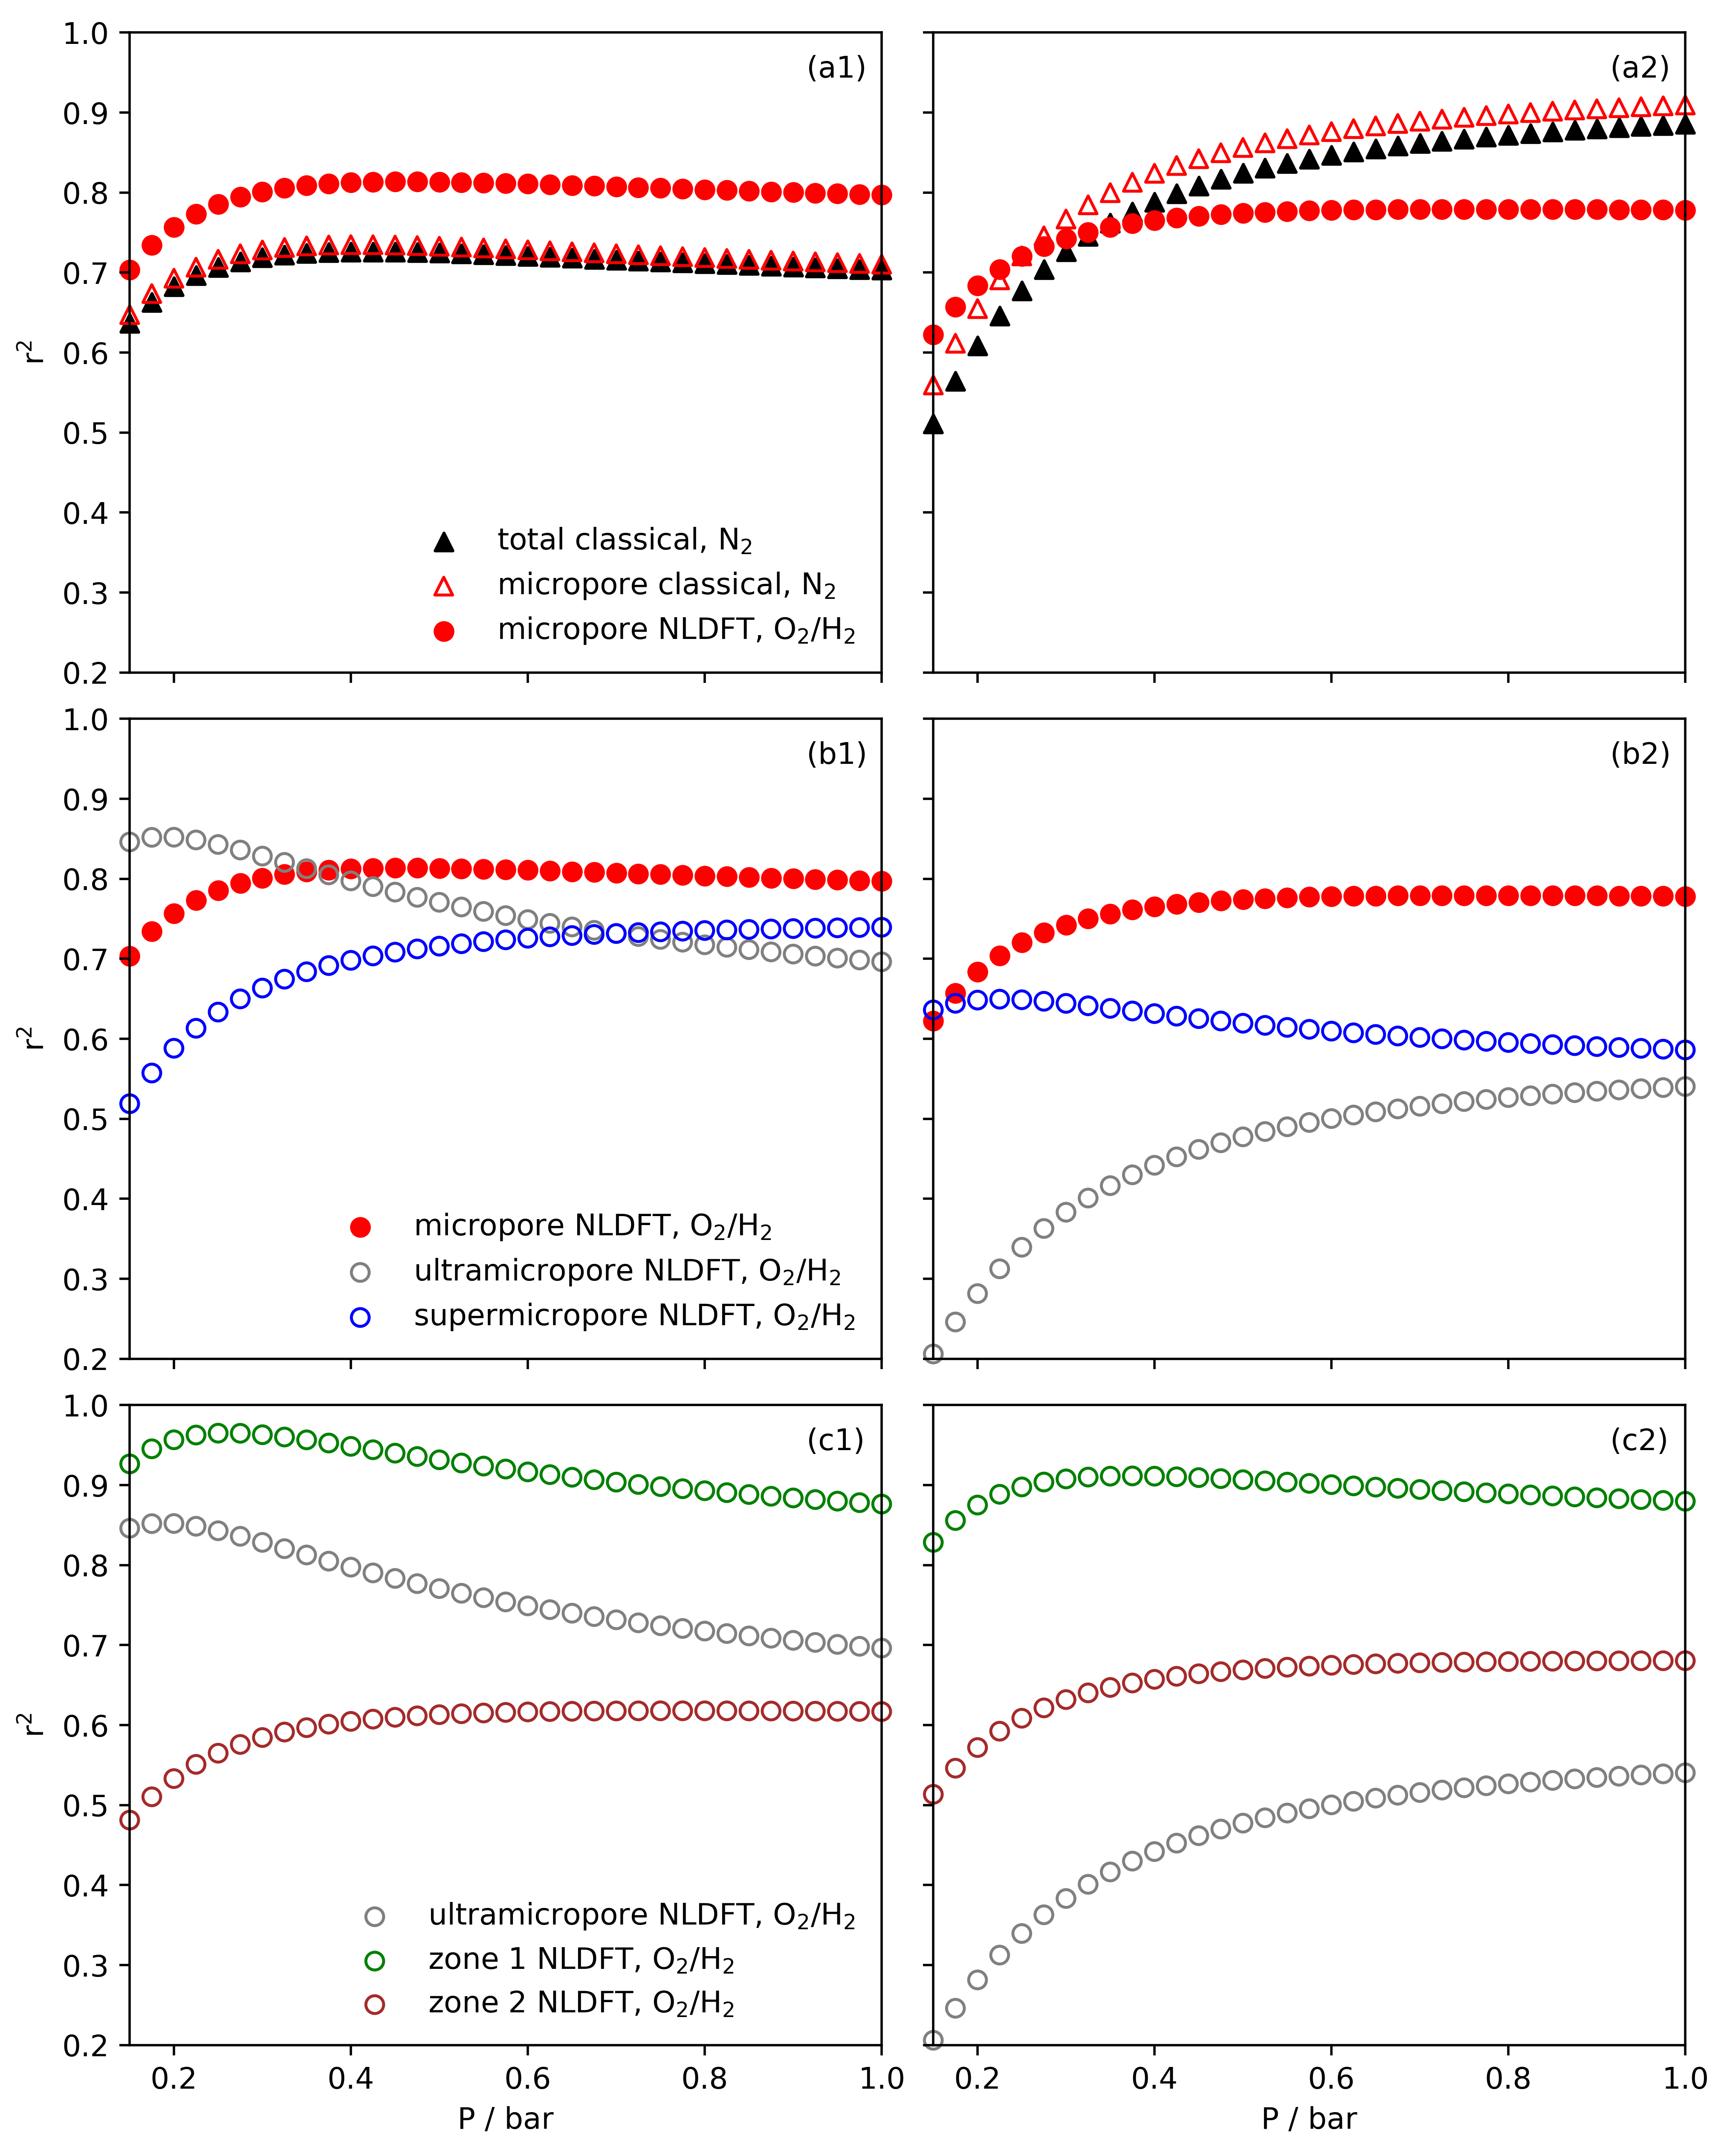
\includegraphics[width=\columnwidth, keepaspectratio]{6-pyPUC/figs/pyPUC_initial.png}
    \caption{Comparison of $r^2$ values derived from the linear regression of porosity as determined by different techniques and within differing pore width ranges against the gravimetric uptake (loading) of \ce{CO2} as a function of pressure. Linear regressions performed with using cumulative \acrshortpl{psd} and \ce{CO2} uptake isotherms of samples from section \ref{s:dual_initial}. Column (1) shows porosity in terms of surface area, and (2) in terms of pore volume. The classical microporosity values in (a1) and (a2) are derived using t-plot, whereas the total porosity is derived using the BET and  single point methods for surface area and pore volume respectively.}
    \label{fig:pyPUC_initial}
\end{figure}

The inconsistent results in terms of surface area and pore volume mentioned above may simply indicate the relative magnitude of the effects which surface area and pore volume of a material have on \gls{adsorption} capacity. Indeed, previous reports have only considered the relationship of pore volume below some pore width with \ce{CO2} uptake.\citep{Presser2011Effect, Sevilla2013Assessment, Adeniran2016Is, Wickramaratne2013Importance} This may be because surface area appears to have a relatively small influence on low pressure \ce{CO2} uptake\citep{Sevilla2021More, Ludwinowicz2015Effect, Singh2019CO2, GrauMarin2020Evaluation}. However, when the \glspl{psd} are subdivided using the variable local minimum technique (see section \ref{s:dual_initial}), the results for both surface area and pore volume are far more consistent as shown in figure \ref{fig:pyPUC_initial}(c1, c2). In other words, both surface area and pore volume in region 1 - that is the pores of widths smaller than the local minimum - are strongly associated with \ce{CO2} uptake at all pressures below \qty{1}{\bar}. In fact $r^2$ values are highest at all pressures using this variable local minimum technique than for any of the other techniques shown in this figure. This indicates that these bimodal \acrshortpl{psd} may have some physical significance to the low-pressure uptake of \ce{CO2}.

In summary, these results indicate that the use of different sorptives can give radically different relationships between \gls{psd} and \ce{CO2} uptake as a function of pressure. This shows further applications of the pyPUC project, as the validity and utility of different porosimetric probes can be thoroughly investigated in their utility for determining optimum pore size range for \ce{CO2} uptake. While initial results are not conclusive, it appears that dual isotherm porosimetry may be important for understanding the relationship between pore size and \ce{CO2} uptake. While the variable local minimum method is impractical, subdividing the \gls{micropore} region at \qty{6.0}{\angstrom} may be more applicable to low pressure \ce{CO2} uptake. This is further investigated in \ref{pub:pyPUC}, \textbf{section 3.2}.

\newpage
\section[Publication II]{\texorpdfstring{Publication II: Brute force determination of the optimum pore sizes for
\ce{CO2} uptake}{Publication III: Brute force determination of the optimum pore sizes for
CO2 uptake}}

\textbf{Contribution of the author}: The author came up with the concept of the pyPUC software, designed and implemented it, and performed all analyses. A portion of the experimental work necessary to create DataSet 1, and all experimental work for DataSet 2 was also done by the author. The author wrote the paper in its entirety.

\setcounter{opagenum}{\thepage}

\newpage

\setlength{\originalVOffset}{\voffset}   
\setlength{\originalHOffset}{\hoffset}

\setlength{\voffset}{0cm}
\setlength{\hoffset}{0cm}
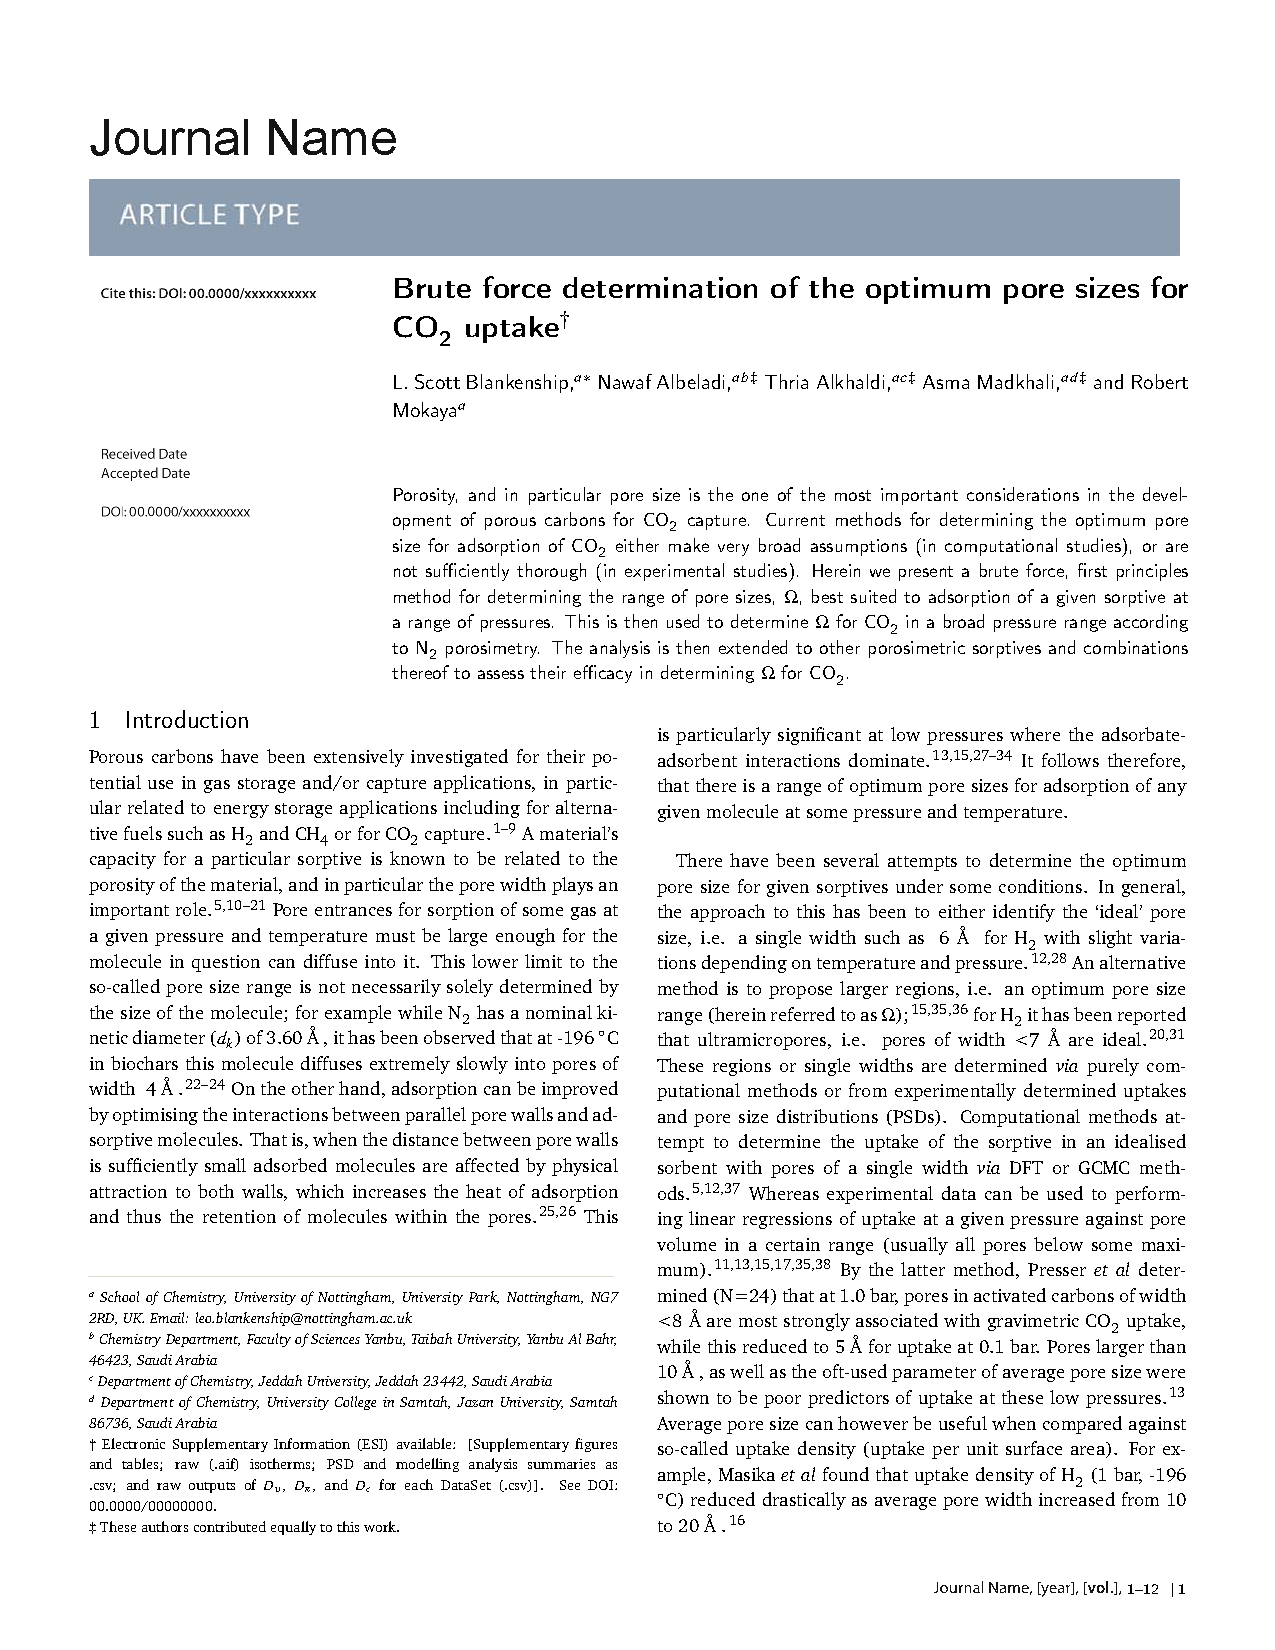
\includepdf[pagecommand={
    \setcounter{page}{\theopagenum}
    \thispagestyle{empty}
    },
    pages=-]{6-pyPUC/publication_03.pdf}
\setlength{\voffset}{\originalVOffset}
\setlength{\hoffset}{\originalHOffset}

%%%%Placeholder
%\section{\texorpdfstring{Describing porosity and pressure dependent \ce{CO2} uptake relationships mathematically}{Describing porosity and pressure dependent CO2 uptake relationships mathematically}}

%\begin{equation}
%    r^2 \left(P,\,w_{max} \right) = \dfrac{A}{P}\exp{\dfrac{\ln{\frac{P}{\mu_g}}}{2\left(\ln{\sigma_g}\right)^2}}
%\end{equation}

%\begin{equation}
%    \sigma_g \left(w_{max}\right) = \sigma_{g(0)}\exp{\left( -\lambda\, w_{max} \right)} + c 
%\end{equation}
%%%%Placeholder

\section{Summary \& Future Work}
The \acrshort{pypuc} method is a thorough, intuitive, and assumption-less route to understanding the relationship between \gls{adsorbent} pore size and physisorptive uptake capacity of some \gls{adsorbate}. It expands upon both purely computational and purely experimental methods by performing a broad analysis of the correlation (\textit{via} the Pearson coefficient, $r^2$) of porosity within pores of some range of widths and \gls{adsorbate} uptake at some pressure. Its utility has been demonstrated in \ref{pub:pyPUC} with \ce{CO2} on \glspl{turbostratic carbon}, with porosity derived from \ce{N2} isotherms as well as by comparing results derived using \acrshortpl{psd} from different porosimetric \glspl{adsorbate}.

The relationship between \ce{CH4} uptake in \glspl{turbostratic carbon} and pore size is one of the least well understood in the field of small gas molecule capture and storage.\citep{Matranga1992Molecular, Tan1990Adsorption, Simon2015materials, Biloe2002Optimal} This problem should be considered a priority for the use of pyPUC - indeed as \ce{CH4} is a non-polar molecule and larger than \ce{CO2},\citep{Breck1974Zeolite, Poling2001Properties} results from this analysis should be less influenced by carbon surface chemistry and very small \glspl{ultramicropore} and thus may provide a simpler understanding of the relationship between pore size and pressure-dependent gas uptake. Similarly pyPUC ought to be applied to \ce{H2} storage; while the relationship between pore size and \ce{H2} uptake capacity is perhaps one of the best understood, the analysis could provide some interesting insights. However, this could be problematic in that the general consensus is that optimum pore size for \ce{H2} uptake is \qty{6.0}{\angstrom}\citep{DelaCasaLillo2002Hydrogen, Cabria2007optimum} so porosity ought to be probed by a small sorptive like \ce{H2} - it could be considered unreasonable to determine porosity with the same molecule for which the materials' uptake capacity is being assessed.

pyPUC currently only considers the uptake capacity in the derivation of the $\Omega$. In the future, pyPUC should be expanded to include isosteric heat of \gls{adsorption} $q_{st}$ as a variable. While $q_{st}$ is typically determined using the Clausius-Clapeyron method,\citep{clausius1850ueber, clapeyron1834memoire} the analysis could perhaps be made more efficient by employing the Whittaker method which has been shown to yield comparable results and only requires a single isotherm.\citep{whittaker2013predicting, li2018adsorption} pyPUC could then be used to derive a relationship between porosity in some range of pore sizes and $q_{st}$.

\newpage
\section[Publication II Supporting Information]{\texorpdfstring{Publication II Supporting Information: Brute force determination of the optimum pore sizes for \ce{CO2} uptake}{Publication III Supporting Information: Brute force determination of the optimum pore sizes for CO2 uptake}}

\setcounter{opagenum}{\thepage}

\newpage

\setlength{\originalVOffset}{\voffset}   
\setlength{\originalHOffset}{\hoffset}

\setlength{\voffset}{0cm}
\setlength{\hoffset}{0cm}
\includepdf[pagecommand={
    \setcounter{page}{\theopagenum}
    \thispagestyle{empty}
    },
    pages=-]{6-pyPUC/si_03.pdf}
\setlength{\voffset}{\originalVOffset}
\setlength{\hoffset}{\originalHOffset}

\bibliographystyle{rsc}
\bibliography{bibliography/bib.bib}